%% This is the ctufit-thesis example file. It is used to produce theses
%% for submission to Czech Technical University, Faculty of Information Technology.
%%
%% Get the newest version from
%% https://gitlab.fit.cvut.cz/theses-templates/FITthesis-LaTeX
%%
%%
%% Copyright 2021, Eliska Sestakova and Ondrej Guth
%%
%% This work may be distributed and/or modified under the
%% conditions of the LaTeX Project Public Licenese, either version 1.3
%% of this license or (at your option) any later version.
%% The latest version of this license is in
%%  https://www.latex-project.org/lppl.txt
%% and version 1.3 or later is part of all distributions of LaTeX
%% version 2005/12/01 or later.
%%
%% This work has the LPPL maintenance status `maintained'.
%%
%% The current maintainer of this work is Ondrej Guth.
%% Contact ondrej.guth@fit.cvut.cz for bug reports.
%% Alternatively, submit bug reports into the tracker at
%% https://gitlab.fit.cvut.cz/theses-templates/FITthesis-LaTeX/issues
%%
%%

%%%%%%%%%%%%%%%%%%%%%%%%%%%%%%%%%%%%%%%%%
% CLASS OPTIONS
% language: czech/english/slovak
% thesis type: bachelor/master/dissertation
%%%%%%%%%%%%%%%%%%%%%%%%%%%%%%%%%%%%%%%%%
\documentclass[english,master,unicode]{ctufit-thesis}

%%%%%%%%%%%%%%%%%%%%%%%%%%%%%%%%%%
% FILL IN THIS INFORMATION
%%%%%%%%%%%%%%%%%%%%%%%%%%%%%%%%%%
\ctufittitle{Math expression evaluator for literal types in TypeScript} % replace with the title of your thesis
\ctufitauthorfull{Bc. Tat Dat Duong} % replace with your full name (first name(s) and then family name(s) / surname(s)) including academic degrees
\ctufitauthorsurnames{Duong} % replace with your surname(s) / family name(s)
\ctufitauthorgivennames{Tat Dat} % replace with your first name(s) / given name(s)
\ctufitsupervisor{Ing.\,Jaroslav Šmolík} % replace with name of your supervisor/advisor (include academic degrees)
\ctufitdepartment{Department of Software Engineering} % replace with the department of your defence
\ctufityear{2023} % replace with the year of your defence
\ctufitdeclarationplace{Prague} % replace with the place where you sign the declaration
\ctufitdeclarationdate{\today} % replace with the date of signature of the declaration
\ctufitabstractCZE{Fill in abstract of this thesis in Czech language. Class aptent taciti sociosqu ad litora torquent per conubia nostra, per inceptos hymenaeos. Cras pede libero, dapibus nec, pretium sit amet, tempor quis. Sed vel lectus. Donec odio tempus molestie, porttitor ut, iaculis quis, sem. Suspendisse sagittis ultrices augue.}
\ctufitabstractENG{Fill in abstract of this thesis in English language. Class aptent taciti sociosqu ad litora torquent per conubia nostra, per inceptos hymenaeos. Cras pede libero, dapibus nec, pretium sit amet, tempor quis. Sed vel lectus. Donec odio tempus molestie, porttitor ut, iaculis quis, sem. Suspendisse sagittis ultrices augue.}
\ctufitkeywordsCZE{enter, commma, separated, list, of, keywords, in, CZECH}
\ctufitkeywordsENG{enter, commma, separated, list, of, keywords, in, ENGLISH}
%%%%%%%%%%%%%%%%%%%%%%%%%%%%%%%%%%
% END FILL IN
%%%%%%%%%%%%%%%%%%%%%%%%%%%%%%%%%%

%%%%%%%%%%%%%%%%%%%%%%%%%%%%%%%%%%
% CUSTOMIZATION of this template
% Skip this part or alter it if you know what you are doing.
%%%%%%%%%%%%%%%%%%%%%%%%%%%%%%%%%%

\RequirePackage{iftex}[2020/03/06]
\iftutex % XeLaTeX and LuaLaTeX
    \RequirePackage{ellipsis}[2020/05/22] %ellipsis workaround for XeLaTeX
\else
    \RequirePackage[utf8]{inputenc}[2018/08/11] %this file encoding
    \RequirePackage{lmodern}[2009/10/30] % vector flavor of Computer Modern font
\fi

% hyperlinks
\RequirePackage[pdfpagelayout=TwoPageRight,colorlinks=false,allcolors=decoration,pdfborder={0 0 0.1}]{hyperref}[2020-05-15]

% uncomment the following to hide all hyperlinks
% \RequirePackage[pdfpagelayout=TwoPageRight,hidelinks]{hyperref}[2020-05-15]

\RequirePackage{pdfpages}[2020/01/28]

\setcounter{secnumdepth}{4} % numbering sections; 4: subsubsection



%%%%%%%%%%%%%%%%%%%%%%%%%%%%%%%%%%
% CUSTOMIZATION of this template END
%%%%%%%%%%%%%%%%%%%%%%%%%%%%%%%%%%


%%%%%%%%%%%%%%%%%%%%%%
% DEMO CONTENTS SETTINGS
% You may choose to modify this part.
%%%%%%%%%%%%%%%%%%%%%%
\usepackage{dirtree}
\usepackage{lipsum,tikz}
\usepackage{csquotes}
\usepackage{inconsolata}
\usepackage{dirtytalk}
\usepackage[style=iso-numeric]{biblatex}
\addbibresource{sources.bib}
% \usepackage{listings} % typesetting of sources
\usepackage[newfloat]{minted} % typesetting of sources
\usepackage{caption}

%theorems, definitions, etc.
\theoremstyle{plain}
\newtheorem{theorem}{Věta}
\newtheorem{lemma}[theorem]{Tvrzení}
\newtheorem{corollary}[theorem]{Důsledek}
\newtheorem{proposition}[theorem]{Návrh}
\newtheorem{definition}[theorem]{Definice}
\theoremstyle{definition}
\newtheorem{example}[theorem]{Příklad}
\theoremstyle{remark}
\newtheorem{note}[theorem]{Poznámka}
\newtheorem*{note*}{Poznámka}
\newtheorem{remark}[theorem]{Pozorování}
\newtheorem*{remark*}{Pozorování}
\numberwithin{theorem}{chapter}
%theorems, definitions, etc. END
%%%%%%%%%%%%%%%%%%%%%%
% DEMO CONTENTS SETTINGS END
%%%%%%%%%%%%%%%%%%%%%%

\onehalfspacing
\newcommand\todo[1]{\textcolor{red}{TODO: #1}}
\NewDocumentCommand{\code}{m}{%
  \texttt{\textcolor{blue}{#1}}%
}

\NewDocumentCommand{\vcode}{v}{%
  \texttt{\textcolor{blue}{#1}}%
}

\begin{document} 
\frontmatter\frontmatterinit % do not remove these two commands

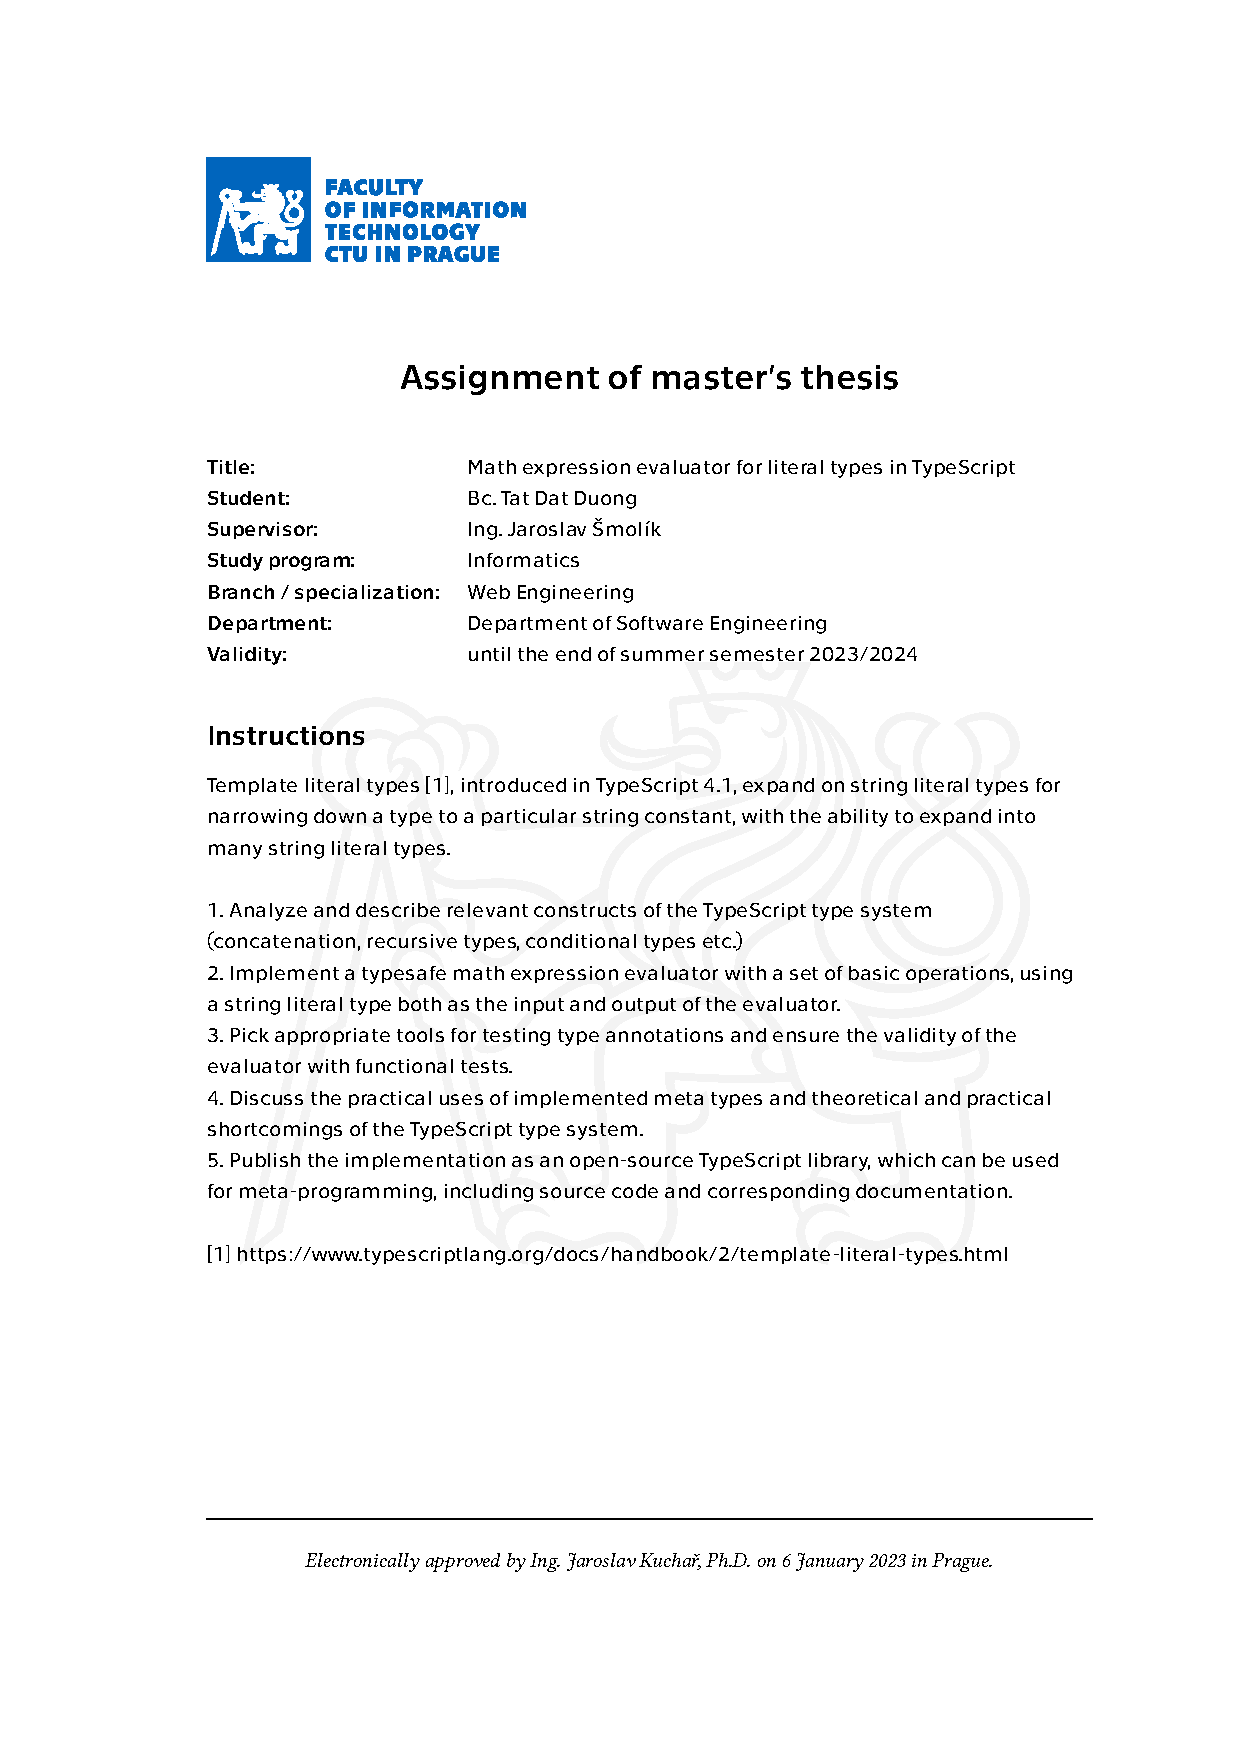
\includepdf{assignment-include.pdf} % replace that file with your thesis assignment provided by study office

\thispagestyle{empty}\cleardoublepage\maketitle % do not remove these three commands

\imprintpage % do not remove this command

\tableofcontents % do not remove this command
%%%%%%%%%%%%%%%%%%%%%%
% list of other contents: figures, tables, code listings, algorithms, etc.
% add/remove commands accordingly
%%%%%%%%%%%%%%%%%%%%%%
\listoffigures % list of figures
\begingroup
\let\clearpage\relax
\listoftables % list of tables
% \lstlistoflistings % list of source code listings generated by the listings package
\listoflistings % list of source code listings generated by the minted package
\endgroup
%%%%%%%%%%%%%%%%%%%%%%
% list of other contents END
%%%%%%%%%%%%%%%%%%%%%%

%%%%%%%%%%%%%%%%%%%
% ACKNOWLEDGMENT
% FILL IN / MODIFY
% This is a place to thank people for helping you. It is common to thank your supervisor.
%%%%%%%%%%%%%%%%%%%
\begin{acknowledgmentpage}
	Chtěl bych poděkovat především sit amet, consectetuer adipiscing elit. Curabitur sagittis hendrerit ante. Class aptent taciti sociosqu ad litora torquent per conubia nostra, per inceptos hymenaeos. Cras pede libero, dapibus nec, pretium sit amet, tempor quis. Sed vel lectus. Donec odio tempus molestie, porttitor ut, iaculis quis, sem. Suspendisse sagittis ultrices augue.
\end{acknowledgmentpage} 
%%%%%%%%%%%%%%%%%%%
% ACKNOWLEDGMENT END
%%%%%%%%%%%%%%%%%%%


%%%%%%%%%%%%%%%%%%%
% DECLARATION
% FILL IN / MODIFY
%%%%%%%%%%%%%%%%%%%
% INSTRUCTIONS
% ENG: choose one of approved texts of the declaration. DO NOT CREATE YOUR OWN. Find the approved texts at https://courses.fit.cvut.cz/SFE/download/index.html#_documents (document Declaration for FT in English)
% CZE/SLO: Vyberte jedno z fakultou schvalenych prohlaseni. NEVKLADEJTE VLASTNI TEXT. Schvalena prohlaseni najdete zde: https://courses.fit.cvut.cz/SZZ/dokumenty/index.html#_dokumenty (prohlášení do ZP)
\begin{declarationpage}
FILL IN ACCORDING TO THE INSTRUCTIONS. VYPLŇTE V SOULADU S POKYNY. Lorem ipsum dolor sit amet, consectetuer adipiscing elit. Curabitur sagittis hendrerit ante. Class aptent taciti sociosqu ad litora torquent per conubia nostra, per inceptos hymenaeos. Cras pede libero, dapibus nec, pretium sit amet, tempor quis. Sed vel lectus. Donec odio tempus molestie, porttitor ut, iaculis quis, sem. Suspendisse sagittis ultrices augue. Donec ipsum massa, ullamcorper in, auctor et, scelerisque sed, est. In sem justo, commodo ut, suscipit at, pharetra vitae, orci. Pellentesque pretium lectus id turpis.

Lorem ipsum dolor sit amet, consectetuer adipiscing elit. Curabitur sagittis hendrerit ante. Class aptent taciti sociosqu ad litora torquent per conubia nostra, per inceptos hymenaeos. Cras pede libero, dapibus nec, pretium sit amet, tempor quis. Sed vel lectus. Donec odio tempus molestie, porttitor ut, iaculis quis, sem. Suspendisse sagittis ultrices augue. Donec ipsum massa, ullamcorper in, auctor et, scelerisque sed, est. In sem justo, commodo ut, suscipit at, pharetra vitae, orci. Pellentesque pretium lectus id turpis.
\end{declarationpage}
%%%%%%%%%%%%%%%%%%%
% DECLARATION END
%%%%%%%%%%%%%%%%%%%

\printabstractpage % do not remove this command

%%%%%%%%%%%%%%%%%%%
% SUMMARY
% FILL IN / MODIFY
% OR REMOVE ENTIRELY (upon agreement with your supervisor)
% (appropriate to remove in most theses)
%%%%%%%%%%%%%%%%%%%
\begin{summarypage}
\section*{Summary section}

\lipsum[1][1-8]

\section*{Summary section}

\lipsum[2][1-6]

\section*{Summary section}

\lipsum[3]

\section*{Summary section}

\lipsum[2]

\section*{Summary section}

\lipsum[1][1-8] Lorem lorem lorem.
\end{summarypage}
%%%%%%%%%%%%%%%%%%%
% SUMMARY END
%%%%%%%%%%%%%%%%%%%

%%%%%%%%%%%%%%%%%%%
% ABBREVIATIONS
% FILL IN / MODIFY
% OR REMOVE ENTIRELY
% List the abbreviations in lexicography order.
%%%%%%%%%%%%%%%%%%%
\chapter{Seznam zkratek}
	
\begin{tabular}{rl}
TC39 & ECMA International, Technical Committee 39\\
W3C & World Wide Web Consortium
\end{tabular}
%%%%%%%%%%%%%%%%%%%
% ABBREVIATIONS END
%%%%%%%%%%%%%%%%%%%

\mainmatter\mainmatterinit % do not remove these two commands

%%%%%%%%%%%%%%%%%%%
% THE THESIS
% MODIFY ANYTHING BELOW THIS LINE
%%%%%%%%%%%%%%%%%%%

\setcounter{page}{1}

\chapter{Introduction}
% \chapter*{Introduction}\addcontentsline{toc}{chapter}{Introduction}\markboth{Introduction}{Introduction}

\section{Motivation}

\section{What is static type system}

In statically typed languages, a data type of a variable is known at compile time. The compiler uses the additional information about data types to verify the source code during compilation. The data type itself can be deduced from the usage in the code (type inferrence) or a programmer explicitly specifies the data type of a variable before usage. Example of such languages using static typing are for instance Java, C\#, C++, etc.

Whereas in dynamically typed languages, the type of a variable is determined at runtime based on the value being assigned. This flexibility allows developers to write code faster in exchange of raised likelihood of type relared errors in runtime. Example of such languages are Python, Ruby, PHP and most notably JavaScript.

Static typing offers numerous compelling benefits, that can enhance the development process:
\begin{itemize}
  \item Reduced likelihood of errors
  \item Self-documenting
  \item Less code to capture intent
  \item More confidence when refactoring
  \item Better tooling
\end{itemize}

First, with static typing a large class of errors are caught much earlier in the development process, thereby reducing the likelihood of bugs and runtime issues, which are inherently harder to catch and debug.

Even though developers might need to write more code to specify the types for the variable, if code is properly structured, the type system is able to determine the intent of the developer without writing additional code.



Additionally, with writing types, developers are actively self-documenting the code, which in turn increases the readability of the code, making the codebase easier to maintain and understand. Refactoring is also significantly easier with static types, as potential errors are raised during compile time instead of runtime.


\section{Cool stuff being done with TS}


\chapter{Analysis}

%---------------------------------------------------------------
\section{Static Typing in JavaScript}
%---------------------------------------------------------------

JavaScript is a dynamically typed programming language, where users do not need to assign types to a variable or a function and the type is inferred automatically by the JavaScript engine. This is a great feature of JavaScript, which lowers the barrier of entry to writing JavaScript code and allows developers to prototype and write code quickly, proven by the growth of popularity of JavaScript in the last decade, making it the most commonly used programming language according to the 2022 Stack Overflow Developer Survey \cite{StackOverflowDeveloper}.

However, dynamic typing has its own drawbacks, as it is harder to spot trivial errors in the code without running it beforehand and it is more difficult to refactor the code without breaking it, which often lead to poor software quality \cite{fardJSNOSEDetectingJavaScript2013a}. Proponents of static typing insist that static types allows developers to spot potential bugs and mistakes earlier during development and that it allows for better tooling, such as more rich code completion and refactoring tools.

There is an upcoming TC39 proposal for adding type annotations, broadly inspired by TypeScript syntax \cite{ECMAScriptProposalType2023}. These annotation are only used for build-time tooling, these annotation are ignored in runtime and the proposal suggests these annotations to be erased by an additional build-step. Even though users can already provide static types using JSDoc right now, the syntax is not as clean as the proposed TypeScript-like syntax.

Regardless, there are many languages which aim to introduce static typing to JavaScript, such as Flow or TypeScript, or alternative languages which compile back to JavaScript, such as Elm or ReScript.

\subsection{Elm}

Elm is a functional programming language designed specifically for building web applications \cite{ElmDelightfulLanguage}. The language compiles to JavaScript and has a strong static Hindley-Milner based type system, which allows to infer types more often and reliably. Elm does not provide any escape hatches such as \code|any| in TypeScript, thus it is harder to write unsafe code, as the types must be valid in order for the code to be compiled.

Elm also includes a lot of quality-of-life improvements and benefits, for instance: enforced purity of functions, out of the box immutability, \code|case| pattern matching, JSON decoders and encoders for strict parsing, \code|Maybe| and \code|Result| monads for avoiding \code|null| and \code|undefined| references or its own virtual DOM implementation for efficient rendering of interactive user interfaces. Notably, the Elm Architecture, where the application code is organized into three parts: model, update and view \cite{ElmArchitectureIntroduction}, has greatly inspired other libraries and frameworks like Redux \cite{PriorArtRedux2022}.

\subsection{ReScript}

ReScript is a programming language built on top of OCaml toolchain. Unlike Flow or TypeScript, ReScript is not a superset of JavaScript, instead the language compiles to JavaScript. ReScript was created as a spin-off from Reason programming language and accompanying BuckleScript compiler, aiming to vertically integrate and streamline the adoption barrier caused by the need to be familiar with multiple unrelated tools and toolchains \cite{BuckleScriptReasonRebranding}.

The language aims to be more sound with more powerful type inference than TypeScript, borrowing the Hindler-Milner type system from OCaml implementation \cite{EfficientInsightfulGeneralization,HistoryReScript2022}, thus most of times the types can be inferred automatically without the need to annotate them explicitly, whereas TypeScript utilizes bidirectional type checking \cite{ReconstructingTypeScriptPart}.

\subsection{Flow}

Flow is a static type checker for JavaScript \cite{chaudhuriFastPreciseType2017,Flow2023}, which allows developers to annotate their code with static types. Flow is developed by Meta and is internally used in production by Facebook, Instagram and React Native. Type annotations in Flow are fully eraseable, which means that the type annotations can be fully removed from the Flow code to emit valid JavaScript code. The checking of these types is occurring at compile-time before removal in build-time. Flow is also a superset of JavaScript, which means any JavaScript code is a valid Flow code.

One the primary goals of Flow is to provide type soundness; the ability to catch every error that might happen in runtime at compile-time, no matter how likely it is to happen. This means, that a valid Flow code can provide developers some guarantees about the type a value has in runtime, at the expense of catching errors, which are unlikely to happen in runtime.

Both Flow and TypeScript are similar in regards to features at the time of writing. Most of the soundness differences between Flow and TypeScript has been addressed with the newer versions of TypeScript, even though soundness is a specific non-goal by the TypeScript team \cite{TypeScriptDesignGoals}. However, developers must opt-in to these features by setting \code|"strict"| to \code|"true"| in \code|tsconfig.json|, whereas in Flow these features are enabled by default.

\subsection{TypeScript}

TypeScript is a staticly typed programming language developed and maintained by Microsoft \cite{TypeScriptJavaScriptSyntax}. It is a language that compiles to JavaScript and adds static type checking to JavaScript \cite{DocumentationTypeScriptJavaScript}. Unlike Elm or ReScript, TypeScript is a syntactical subset of JavaScript, which means that any valid JavaScript code can be a valid TypeScript code\footnote{With a lax compiler configuration}. Similar to Flow, type annotation provided by the developer are fully eraseable either by the TypeScript \code|tsc| compiler or by other community build tools, such as \code|babel|\cite{BabelCompilerNext}, \code|esbuild|\cite{EsbuildExtremelyFast} or \code|swc|\cite{SWCRustbasedPlatform}.

Type system in TypeScript is considered to be less sound and more forgiving, as soundness is stated as an explicit non-goal for the design team of TypeScript \cite{TypeScriptDesignGoals}, emphasis on striking a balance between productivity and correctness. By default, TypeScript compiler is not strict and the language itself includes an escape hatch for developers to opt-out of type checking by using the \code|any| type or using \code|@ts-ignore| comment annotations. Nevertheless, with proper compiler configuration, the type system of TypeScript can be as sound as in Flow.

Both Flow and TypeScript support advanced features such as generics and utility types, with the latter supporting template string literal types and better support for conditional types, unlocking the potential of writing more expressive types, which this master thesis will further explore in more detail.

TypeScript has become the de-facto standard for writing JavaScript code with static types. With deep integration with Visual Studio Code \cite{VisualStudioCode}, rich build ecosystem and high compatibility with existing JavaScript libraries and tools, TypeScript has become one of the fastest growing language according to 2022 Octoverse report by Github \cite{Octoverse2022State}.

\section{Typescript syntax}


\subsection{Types and their assignability}

\begin{itemize}
  \item Primitive Types
  \item Literal Types
  \item \code{unknown}, \code{never}, \code{any}
  \item Structures (nominal vs structural typing)
  \item Unions and Intersections
\end{itemize}

\subsection{Conditional Types}
\subsection{Recursive Types}
\subsection{Mapped Types}
\subsection{Template Literal Types}

\section{Prior Art}

\begin{itemize}
  \item \code{kawayiLinLin/typescript-lodash}
  \item \code{arielhs/ts-arithmetic}
  \item \code{ts-belt}
  \item \code{type-fest}
\end{itemize}

\chapter{Implementation}

\section{Structure of the project}
\section{Type representation of numbers}
\section{Addition and Subtraction}
\section{Multiplication}
\section{Division}
\section{Exponentiation}
\section{Other mathematical operations}
\section{Statement parser \& evaluator}
\section{Higher kinded types}
\section{Optimization and bypasses}

\chapter{Testing}

\section{Developer experience}

By using \code{tsserver}, we can see and verify the types representing a symbol during development, by hovering on top of a symbol. This does provide some useful feedback during development but does require significant context switching with the mouse pointer, especially when switching back and forth from implementation to testing. There are various plugins for editors, that are able to display the inferred types in a different manner. One such key plugin used thoroughly during development is \code{vscode-twoslash-plugins} \cite{theroxVscodetwoslashqueries2023}, which allows inserting a \code{// ^?} comment to display the inferred type of an expression right in the editor.

\todo {Add a screenshot of the vscode-twoslash-plugins in action}

\section{Testing with eslint}

\todo {Describe \$ExpectType}

To remedy the issue, we are using \code{eslint} together with \code{@typescript-eslint/parser} as the source code parser and \code{eslint-plugin-expect-type} plugin to create unit tests for each of the math methods.

\begin{itemize}
  \item Developer experience
  \item Unit tests, integration tests (\code{eslint}, \code{eslint-plugin-expect-type})
  \item Github Actions
  \item Performance Testing (performance tracing, extended diagnostics)
  \item Comparison between existing TS math libraries
\end{itemize}

\chapter{Conclusion}

This thesis set out to implement a mathematical expression evaluator entirely written in the type system of TypeScript. Core concepts and techniques of TypeScript type-level programming were introduced and explained. The implementation of the expression evaluator was described in detail, and the implementation was evaluated in terms of correctness and performance using type-level unit tests and benchmarking suites.

The created evaluator is a proof-of-concept, demonstrating the capabilities of the TypeScript type system while addressing some of the limitations of the type system by applying workarounds.

This thesis also provides a comprehensive guide to the TypeScript syntax and type system and can be used as a reference for beginners to the type-level programming in TypeScript. Additional tools and utility types were introduced to aid the development of the mathematical evaluator, namely the benchmarking tool and the LL(1) parser generator.

The rest of this chapter will discuss both the practicality of the created types and the limitations of the type system found during development. Finally, the future work will be outlined.

\section{Practical usage}

The TypeScript type system is powerful for static type-checking and inference. However, it is not without its limitations. These advanced types are considered to be extreme and are generally not recommended to be used in production code, as they can severely impact the compilation time and the in-editor developer experience.

Nevertheless, there are some possible practical use cases for these advanced types. Literal types are often used to describe a design system and accompanying design tokens. Namely, numeric literal types are used to describe the spacing and sizing of components. When the spacing is defined in other units, such as \code{rem} or \code{em}, developers often need to manually convert the values into pixels. A utility type can be introduced to convert values in \code{rem} or \code{em} units into pixels and reverse. This can be further expanded to allow more type transformations, such as converting a Tailwind CSS class name into a CSS string without any TypeScript editor plugins.

The parser and the accompanying parser generator can accept any LL(1) grammar and can be used to parse more complex formats, such as JSON. Finally, the benchmarking tool can be used to benchmark any type-level code in isolation, keeping all the test cases in a single file.

\section{Limitations of the TypeScript type system}

When developing the implementation of the evaluator, some limitations of the TypeScript type system were discovered.

In general, error messages in TypeScript are suboptimal. They tend to be displayed in one line without any formatting, and if they include complicated types, the types are truncated, which leads to a suboptimal debugging experience. Even with \code{noErrorTruncation} flag turned on in \code{tsconfig.json}, the type message is still truncated due to a hard limit. The limit can be artificially raised by patching the TypeScript source code, namely by increasing the \code{defaultMaximumTrucationLength} limit, but this is not a viable solution for production code. The only other option is to manually recreate intermediate types when debugging complicated types.

The type checker itself contains many hardcoded constraints to prevent performance degradation, ranging from the maximum tuple size to the limit on both instantiation count and depth. Some checks can be bypassed using various workarounds, often at a performance cost, discussed in previous chapters. However, these workarounds are poorly documented in the official TypeScript documentation and can break with new TypeScript releases without further notice.

Even though the TypeScript type system is powerful for complex types, some highly requested features are still missing as of the writing of this thesis, such as the lack of partial type argument inference \cite{ImplementPartialType} or lack of built-in utility types for type-level assertions. Some of these features can be partially emulated, such as the lack of higher kinded types, but the behaviour can also change with new TypeScript releases.

Finally, as the type checker itself is written in TypeScript to dogfood the language, it can be inherently slow when working with larger TypeScript codebases. Some of these performance issues are being solved by rewriting the type checker in a different programming language, such as Rust \cite{Stc2023}, but the project is still under active development.

\section{Future work}

Most of the future work is geared towards the underlying tooling and utilities rather than the mathematical expression evaluator itself, which can be further extended by adding additional mathematical operations based on the existing utility types implemented in this thesis.

For instance, the LL(1) parser generator is not flexible enough, as it can only generate code for LL(1) grammars, which, while being sufficient for mathematical expressions and other simple formats such as JSON, is not enough for more complex grammars. Future work could include creating a more generic Look-Ahead LR parser generator, which would be able to parse more complex grammars and programming languages.

The benchmarking utility itself can be extended and packaged both as an \acrshort{npm} package and as a GitHub Action. This is especially useful for library maintainers, which can use the additional CI step to monitor potential performance regressions when reviewing pull requests from contributors.


\appendix\appendixinit % do not remove these two commands

\chapter{Performance measurements}\label{appendix:performance}

\begin{table}
  \begin{tabular}{lll}
    \toprule
    {}                                     & Instantiation Count & Check Time (ms)          \\
    \midrule
    \code{Add<"1", "1">}                   & 50389               & $626.1480 \pm 2732.4835$ \\
    \code{Add<"1", "10">}                  & 50541               & $608.1964 \pm 1490.2754$ \\
    \code{Add<"1", "100">}                 & 50637               & $628.2837 \pm 1187.9201$ \\
    \code{Add<"1", "1000">}                & 50734               & $590.4544 \pm 1323.4114$ \\
    \code{Add<"1", "10000">}               & 50833               & $563.4551 \pm 503.1991$  \\
    \code{Add<"1", "100000">}              & 50934               & $564.6383 \pm 326.1892$  \\
    \code{Add<"1", "1000000">}             & 51037               & $590.2288 \pm 800.6683$  \\
    \code{Add<"1", "10000000">}            & 51142               & $566.8994 \pm 1322.4848$ \\
    \code{Add<"1", "100000000">}           & 51249               & $592.8983 \pm 2703.7284$ \\
    \code{Add<"1", "1000000000">}          & 51358               & $580.8956 \pm 732.7624$  \\
    \code{Add<"1", "10000000000">}         & 51469               & $602.9816 \pm 2772.3885$ \\
    \code{Add<"1", "100000000000">}        & 51582               & $574.9316 \pm 443.2602$  \\
    \code{Add<"1", "1000000000000">}       & 51714               & $573.1765 \pm 288.5311$  \\
    \code{Add<"1", "10000000000000">}      & 51849               & $593.7831 \pm 815.4532$  \\
    \code{Add<"1", "100000000000000">}     & 51987               & $576.2892 \pm 1581.0826$ \\
    \code{Add<"1", "1000000000000000">}    & 52128               & $564.1985 \pm 226.5942$  \\
    \code{Add<"1", "10000000000000000">}   & 52272               & $561.8088 \pm 202.4868$  \\
    \code{Add<"1", "100000000000000000">}  & 52419               & $588.9620 \pm 1605.4446$ \\
    \code{Add<"1", "1000000000000000000">} & 52569               & $598.1670 \pm 2184.9193$ \\
    \bottomrule
  \end{tabular}
  \caption{Instantiation count and check time for \code{Add}}
  \label{tab:appendix:add}
\end{table}

\begin{table}
  \begin{tabular}{lll}
    \toprule
    {}                                          & Instantiation Count & Check Time (ms)          \\
    \midrule
    \code{Multiply<"1", "1">}                   & 52418               & $566.2856 \pm 1304.8233$ \\
    \code{Multiply<"1", "10">}                  & 52742               & $586.9069 \pm 2054.9946$ \\
    \code{Multiply<"1", "100">}                 & 53057               & $548.8409 \pm 291.8180$  \\
    \code{Multiply<"1", "1000">}                & 53436               & $552.7645 \pm 1010.9699$ \\
    \code{Multiply<"1", "10000">}               & 53879               & $573.1269 \pm 1982.9075$ \\
    \code{Multiply<"1", "100000">}              & 54383               & $552.6068 \pm 404.8264$  \\
    \code{Multiply<"1", "1000000">}             & 54948               & $543.9872 \pm 156.1134$  \\
    \code{Multiply<"1", "10000000">}            & 55574               & $552.3896 \pm 391.9594$  \\
    \code{Multiply<"1", "100000000">}           & 56261               & $569.8469 \pm 1450.4120$ \\
    \code{Multiply<"1", "1000000000">}          & 57009               & $582.6160 \pm 2282.8004$ \\
    \code{Multiply<"1", "10000000000">}         & 57818               & $588.8492 \pm 2708.3371$ \\
    \code{Multiply<"1", "100000000000">}        & 58705               & $571.0721 \pm 1108.1628$ \\
    \code{Multiply<"1", "1000000000000">}       & 59654               & $561.9530 \pm 502.5156$  \\
    \code{Multiply<"1", "10000000000000">}      & 60665               & $586.2230 \pm 1929.5835$ \\
    \code{Multiply<"1", "100000000000000">}     & 61738               & $582.3424 \pm 1791.3684$ \\
    \code{Multiply<"1", "1000000000000000">}    & 62873               & $594.4613 \pm 2638.3184$ \\
    \code{Multiply<"1", "10000000000000000">}   & 64070               & $586.1715 \pm 1270.7923$ \\
    \code{Multiply<"1", "100000000000000000">}  & 65329               & $580.8701 \pm 641.9969$  \\
    \code{Multiply<"1", "1000000000000000000">} & 66650               & $587.0313 \pm 1519.6371$ \\
    \bottomrule
  \end{tabular}
  \caption{Instantiation count and check time for \code{Multiply}}
  \label{tab:appendix:multiply}
\end{table}

\begin{table}
  \begin{tabular}{lll}
    \toprule
    {}                                        & Instantiation Count & Check Time (ms)          \\
    \midrule
    \code{Divide<"1", "3">}                   & 56065               & $611.1183 \pm 3712.1221$ \\
    \code{Divide<"10", "3">}                  & 56007               & $566.6266 \pm 1312.9779$ \\
    \code{Divide<"100", "3">}                 & 56190               & $554.2810 \pm 178.3204$  \\
    \code{Divide<"1000", "3">}                & 56257               & $545.5406 \pm 1368.3422$ \\
    \code{Divide<"10000", "3">}               & 56317               & $552.3237 \pm 1120.0729$ \\
    \code{Divide<"100000", "3">}              & 56377               & $579.1138 \pm 841.8474$  \\
    \code{Divide<"1000000", "3">}             & 56437               & $590.3914 \pm 2730.2088$ \\
    \code{Divide<"10000000", "3">}            & 56497               & $552.0362 \pm 983.1479$  \\
    \code{Divide<"100000000", "3">}           & 56557               & $552.2182 \pm 1549.2122$ \\
    \code{Divide<"1000000000", "3">}          & 56617               & $576.9744 \pm 1538.6618$ \\
    \code{Divide<"10000000000", "3">}         & 56677               & $584.4138 \pm 1771.3998$ \\
    \code{Divide<"100000000000", "3">}        & 56767               & $575.2797 \pm 2817.7110$ \\
    \code{Divide<"1000000000000", "3">}       & 56875               & $574.0339 \pm 1187.0906$ \\
    \code{Divide<"10000000000000", "3">}      & 56985               & $572.9396 \pm 1845.7412$ \\
    \code{Divide<"100000000000000", "3">}     & 57097               & $544.0291 \pm 187.0663$  \\
    \code{Divide<"1000000000000000", "3">}    & 57211               & $610.6468 \pm 1628.6978$ \\
    \code{Divide<"10000000000000000", "3">}   & 57327               & $597.4917 \pm 751.0289$  \\
    \code{Divide<"100000000000000000", "3">}  & 57445               & $549.7234 \pm 404.5449$  \\
    \code{Divide<"1000000000000000000", "3">} & 57565               & $580.1838 \pm 1396.0654$ \\
    \bottomrule
  \end{tabular}

  \caption{Instantiation count and check time for \code{Divide}}
  \label{tab:appendix:divide}
\end{table}

\begin{table}
  \begin{tabular}{lll}
    \toprule
    {}                                      & Instantiation Count & Check Time (ms)             \\
    \midrule
    \code{Root<"1", "2">}                   & 101781              & $657.9258 \pm 4637.2670$    \\
    \code{Root<"10", "2">}                  & 943579              & $2231.2624 \pm 26354.7449$  \\
    \code{Root<"100", "2">}                 & 995709              & $2358.4428 \pm 46642.8882$  \\
    \code{Root<"1000", "2">}                & 1150338             & $2457.2318 \pm 7974.3022$   \\
    \code{Root<"10000", "2">}               & 1290084             & $2717.1363 \pm 22569.9561$  \\
    \code{Root<"100000", "2">}              & 1390432             & $3114.9099 \pm 89929.3402$  \\
    \code{Root<"1000000", "2">}             & 1480678             & $3476.8778 \pm 132963.1171$ \\
    \code{Root<"10000000", "2">}            & 1715701             & $3535.6702 \pm 217462.3269$ \\
    \code{Root<"100000000", "2">}           & 1944285             & $4017.5913 \pm 22143.6082$  \\
    \code{Root<"1000000000", "2">}          & 2264897             & $4512.2763 \pm 45757.7304$  \\
    \code{Root<"10000000000", "2">}         & 2614395             & $5477.2640 \pm 64109.5688$  \\
    \code{Root<"100000000000", "2">}        & 2898459             & $6333.6284 \pm 9891.4644$   \\
    \code{Root<"1000000000000", "2">}       & 3157392             & $6439.0302 \pm 36044.4666$  \\
    \code{Root<"10000000000000", "2">}      & 3400798             & $6758.4044 \pm 84619.0587$  \\
    \code{Root<"100000000000000", "2">}     & 3630962             & $6763.4433 \pm 32105.0016$  \\
    \code{Root<"1000000000000000", "2">}    & 3861157             & $7483.2405 \pm 52541.9327$  \\
    \code{Root<"10000000000000000", "2">}   & 4087750             & $7638.8097 \pm 163773.6981$ \\
    \code{Root<"100000000000000000", "2">}  & 4319968             & $8199.8814 \pm 306798.3177$ \\
    \code{Root<"1000000000000000000", "2">} & 4558096             & $8563.6442 \pm 363040.7800$ \\
    \bottomrule
  \end{tabular}

  \caption{Instantiation count and check time for \code{Root}}
  \label{tab:appendix:root}
\end{table}
 % include `appendix.tex' from `text/' subdirectory

\backmatter % do not remove this command

\printbibliography % print out the BibLaTeX-generated bibliography list

\chapter{Contents of the attached media}


\dirtree{%
.1 .changeset.
.2 config.json\DTcomment{Configuration file for Changesets}.
.1 .github.
.2 workflows.
.3 main.yml\DTcomment{Continuous integration and testing}.
.3 publish.yml\DTcomment{Automatic publishing to \acrshort{npm} registry}.
.1 .vscode\DTcomment{Common configuration for VSCode}.
.1 assets\DTcomment{Assets for \acrshort{npm} and GitHub README}.
.1 benchmark\DTcomment{JSON benchmarking results}.
.1 scripts.
.2 bench.ts\DTcomment{Benchmarking script}.
.2 dirtree.ts\DTcomment{Generator of LaTeX dirtree}.
.2 generate.ts\DTcomment{Lookup table generation}.
.2 parser.ts\DTcomment{LL(1) parser generator}.
.1 src\DTcomment{Source code of the implementation}.
.2 expression\DTcomment{Expression evaluator}.
.2 math\DTcomment{Mathematical operations}.
.2 utils\DTcomment{Utility functions}.
.1 thesis\DTcomment{Source code for the thesis}.
}
 % include `medium.tex' from `text/' subdirectory

\end{document}